One can see an example of what Golgi fluorescence staining looks like in Figure \ref{fig:golgi-enhancement}. It is evident that there is a lighter foreground fluorescence and slightly darker one in the background. A true Golgi signal here is considered to be only the lighter part of fluorescence lighting. The light gray background present here is called a non-specific fluorescence lighting. It comes from the cell itself, and might occur when the antigen is impure and contains antigenic contaminants (\cite{Borek_1984}). Its brightness may vary due to longer or shorter exposure times. 

\begin{figure}[htb]
	\begin{center}
		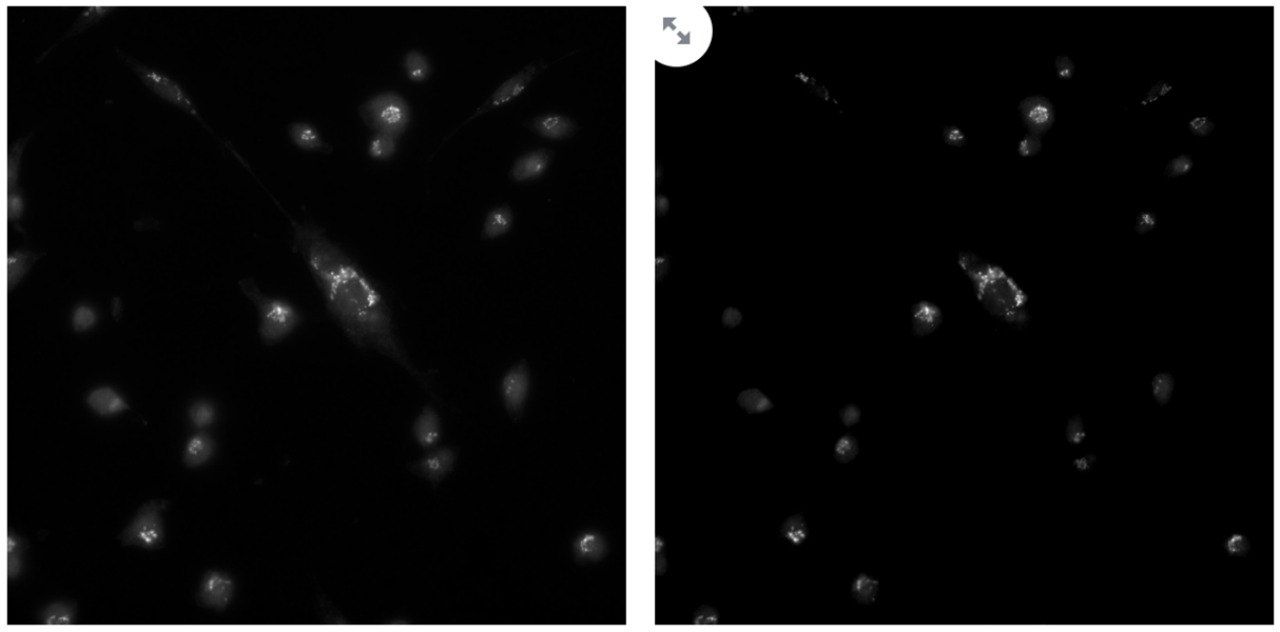
\includegraphics[width=0.5\linewidth]{bilder/enhancement.jpg}
		\caption{Golgi enhancement: left --- original signal, right --- enhanced image}\label{fig:golgi-enhancement}
	\end{center}
\end{figure}

Having such a non-specific fluorescence background has two challenges for training:
\begin{itemize}
    \item The relative area of the background fluorescence is bigger than the area of Golgi themselves. Therefore quite a big part of the loss during training will be dedicated to teaching the model to restore this background fluorescence instead of the Golgi itself.
    \item It introduces difficulties during the postprocessing of the predictions. As well as for nuclei, the mask of the predicted Golgi apparatus is needed for further evaluation of the downstream metrics. Using the same algorithm for postprocessing segmentation that was used for nuclei, the mask of the Golgi Apparatus will consider the background noise to be relevant, although this is an unwanted behavior.
\end{itemize}

In the left part of Figure \ref{fig:golgi-enhancement} one can see the original ground truth image and on the right side we can see the images after the background was subtracted. One of the great background subtraction algorithms is the rolling ball algorithm which is described below.

Additionally, all of the crops used for training were filtered base on the amount of background they contain. Without filtering the crops that contain a lot of background, a big portion of a dataset would consist of black crops only, which creates very strong class imbalance.
